\documentclass[12pt,a4paper]{article}

\usepackage[utf8]{inputenc}
\usepackage{graphicx}
\usepackage{pdfpages}
\usepackage{csquotes} % czech styled quotes 
\usepackage[czech]{babel} % czech babel 
\usepackage{mathtools} % math magic
\usepackage{amssymb} % some funky math symbols like \trinangleq
\usepackage[left=4cm,right=1.5cm,top=3cm,bottom=3cm]{geometry} % set smaller page borders 
\usepackage[indent=0pt]{parskip} % spaces between paragraphs, indents sets indent of the first line in paragraph
\usepackage[hidelinks]{hyperref}
\usepackage{pdflscape}
\usepackage{enumitem}
\usepackage{caption}
\usepackage{subcaption}
\usepackage{fontspec}
\usepackage{unicode-math}
\usepackage{lmodern}
\usepackage{setspace}
\usepackage{titlesec}
\usepackage{float}

\usepackage{tocloft}

\usepackage{listings}
\usepackage{color}

% Add dots for sections and subsections in the table of contents
\renewcommand{\cftsecleader}{\cftdotfill{\cftdotsep}} % for sections
\renewcommand{\cftsubsecleader}{\cftdotfill{\cftdotsep}} % for subsections

\definecolor{dkgreen}{rgb}{0,0.6,0}
\definecolor{gray}{rgb}{0.5,0.5,0.5}
\definecolor{mauve}{rgb}{0.58,0,0.82}

\lstset{
	language=Python,
	showstringspaces=false,
	columns=flexible,
	basicstyle={\small\ttfamily},
	numbers=none,
	numberstyle=\tiny\color{gray},
	keywordstyle=\color{blue},
	commentstyle=\color{dkgreen},
	stringstyle=\color{mauve},
	breaklines=true,
	breakatwhitespace=true,
	tabsize=4
}

\setstretch{1.5}
\setmainfont[
	Extension=.otf,
	UprightFont={*-Regular},
	BoldFont={*-Bold},
	ItalicFont={*-Italic},
	BoldItalicFont={*-BoldItalic},
	% RawFeature={+zero}
]{LibertinusSerif}
\setmathfont{LibertinusMath-Regular.otf}

\graphicspath{{images/}}


\begin{document}


\includepdf[pages=-]{add_files/mp_titlelist}
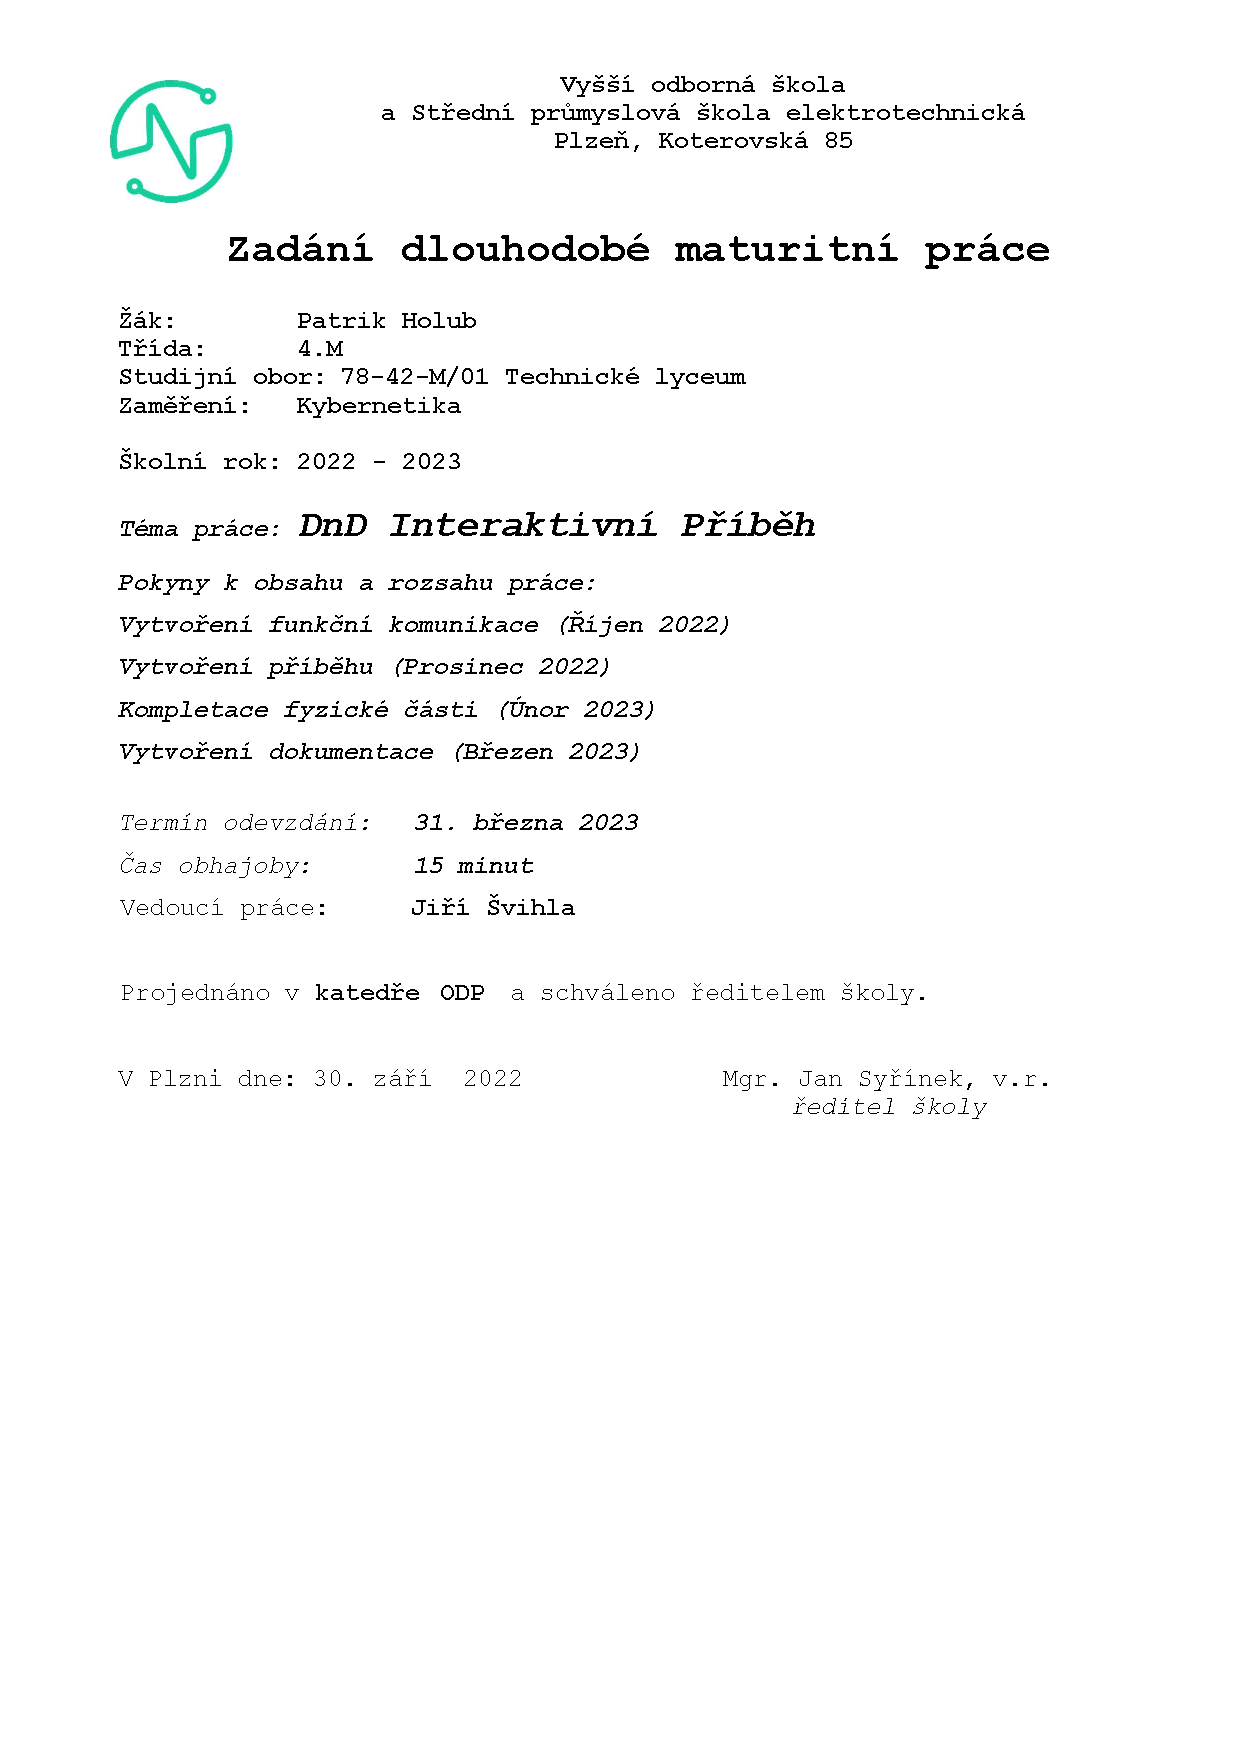
\includepdf[pages=-]{add_files/zadanibelike}

\newpage

\section*{Anotace}
V této maturitní práci se snažím o vytvoření programu který je schopný přednést příběh a předložit hráči možnosti na které příběh bude reagovat. Tímto se docílí interaktivita příběhu. Zároveň vše je děláno systémem skriptů, tudíž je možno hru, při dodržení pravidel pro psaní daných skriptů, měnit pomocí uživatelsky napsaných programů. Projekt také obsahuje metodu se kterou se dá zjednodušeně příběh napsat a použít jednotlivé skripty pro interaktivitu. Poslední část práce je uložení hráče a jeho odpovídajících skriptů na raspberry pi pico a čtení předem zmíněného obsahu ze zařízení. Celá práce je dělaná v programovacím jazyku Micropython.
%\addcontentsline{toc}{Anotace}{Anotace}


\vspace*{\fill}

„Prohlašuji, že jsem tuto práci vypracoval samostatně a použil(a) literárních pramenů a informací, které cituji a uvádím v seznamu použité literatury a zdrojů informací.“ 
„Souhlasím s využitím mé práce učiteli VOŠ a SPŠE Plzeň k výuce.“ 
\begin{flushright}
	V Plzni dne: …..................... Podpis: …..........................
\end{flushright} 

\newpage
\tableofcontents
\newpage

\addcontentsline{toc}{section}{Úvod}
\section*{Úvod}
Jako první bych rád vysvětlil pojem DnD, abychom dál věděli k čemu jsem se snažil dostat. 

DnD je stolní skupinová hra. Skupinová pouze proto, protože v jednom se tomu říká psaní knihy. Mezi hráči je jeden vypravěč a standardně více hráčů. Vypravěč si připraví příběh a svět, který svým hráčům bude přednášet a ve kterém je bude provádět. Když začne hrát tak se v určitých momentech ptá hráčů jak se chtějí zachovat, či co chtějí dělat. Po tom co hráči zvolí, tak si hodí kostkou aby zjistili jestli se jim daná akce povedla. Na základě tohoto výsledku vypravěč improvizací vytvoří novou část příběhu. Takto se celý příběh rozvíjí až snad někdy skončí.

Improvizace je ve světe DnD jedna z nejdůležitějších schopností. Bohužel počítače nejsou dobré v kreativitě. Tudíž, pokud jako programátoři chceme vytvořit hry s námětem DnD, musíme se velmi snažit. Já jsem rozhodl pro textově založenou hru, neboť má relativně jednoduché prostředí. Vím že nejsem výborný programátor a proto jsem věděl že tvorba takové hry pro mne bude obtížná. Nakonec jsem se ustálil s tím, že vytvořím hru, která bude lehká hrát pro hráče a bude mít nástroje pro lehké tvoření příběhu pro vypravěče. Není to přesné vytvoření DnD, ale je to dobrý začátek, ze kterého se dá posunout dál.

Aby šel příběh psát jednoduše a aby mohly příběhy být rozmanité, tak jsem se rozhodl pro hru, která bude možná rozšířit pomocí skriptů. Aby vypravěč nemusel umět programovat, tak jsem také chtěl udělat zjednodušený zápis pro program, víceméně DSL. Další část byla nějak vytvořit určitou nutnost socializace mezi hráči. Jinak řečeno, chtěl jsem aby se hráči scházeli, aby nemohli hru hrát online. Proto jsem musel vytvořit nějakou fyzickou část, která by toto vyvolala. Napadl mě fyzický klíč, ke kterému se blíž vyjádřím v jeho odpovídající sekci.

\newpage
\section{Fyzický klíč}
Při prvotním plánu práce jsem chtěl přidat určitou interaktivitu k hlavnímu programu z nějakého zařízení. Napadly mě dvě myšlenky, které jsem spojil dohromady. První byla že pokud bude hlavní program hra, kde mohou hráči prozkoumávat různé podzemní komnaty, tak by mohlo zařízení být nějaký klíč. Druhá myšlenka byla, aby hráči mohli jednoduše přenášet postavy a neměli strach že se jim smažou v rukou vypravěče, tak bych mohl utvořit něco co by fungovalo jako úložné zařízení.

Nakonec jsem se rozhodl pro desku založenou na čipu RP2040, protože existuje docela dobrá dokumentace k tvorbě vlastních desek. Samotná dokumentace k čipu je velmi hustá a technická a pro moje účely zbytečně složitá. Druhý důvod proč zvolit čip RP2040 bylo, že je na desce Raspberry Pi Pico a Pico W. Tyto dvě desky jsem používal pro programování čipu v jazyce Micropython a vytváření velké čísti programu dřív než jsem dokončil vlastní PCB. Třetí důvod, který není tak důležitý, je že tento čip je relativně silný v rámci výpočetní schopnosti a tudíž jsem nemusel řešit hlubokou optimalizaci. Když jsem zjistil jak velká porce mé práce byl hlavní program, tak jsem za tyto vlastnosti byl velmi vděčný.

Nakonec zvolenou interaktivitou bylo, že klíč bude schopen zobrazit nějaké informace ohledně hráče. Zobrazovací metodu jsem vybral řady osmi LED. Nechtěl jsem ale aby zabrali 16 pinů na čipu a tudíž mě napadlo řešení přes registry. Tím bych byl schopen snížit počet pinů na 8. Avšak učitel mě navedl na ještě úspornější cestu. Nakonec jsem použil jenom jeden registr připojený k oběma řadám. Každá řada má tranzistor s otevřeným kolektorem, tudíž uzemňuje. Aby obě řady svítily stejně, tak je následně přepíná s intervalem 100 milisekund. Tímto se vytvořil časový multiplex.

Diody jsou napájeny přímo z registru, který je napájen z usb neboli 5 volty. Elektronické zapojení je vidět na Obrázku 1. Hodnoty rezistorů závisí na napětí zvolených LED a ty které jsem zvolil vyžadovali tyto rezistory. Celé schéma zapojení je následně v Příloze 1.

\begin{figure}[H]
    \centering
    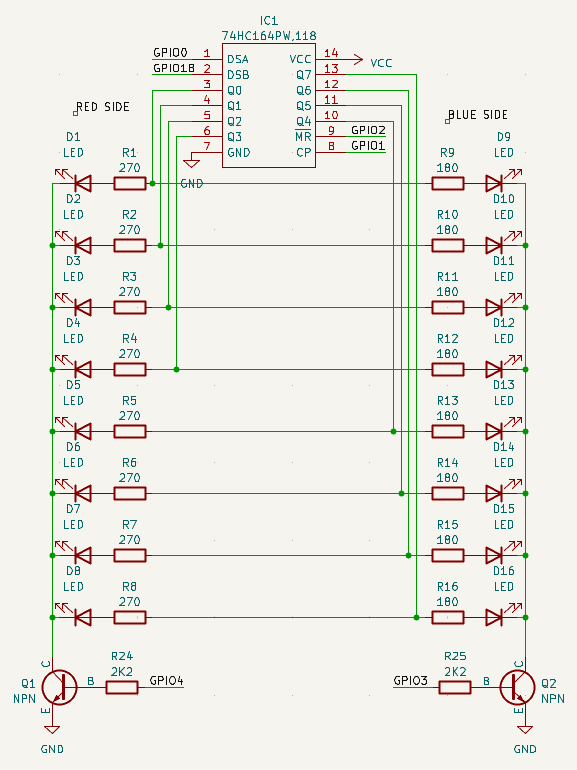
\includegraphics[width=\textwidth-3 cm]{pictures/register_LED.png}
    \caption{Registr a LED řady [vlastní]}
\end{figure}

Ve hlavním schéma je kromě zapojení paměti a filtrování také jedna RGB LED. Takto led je určená převážně pro debug. Tento nápad jsem měl kvůli existenci vestavěné zelené LED na Raspberry Pi Pico, která se často pro tyto účely používá. Nicméně je to pouze jednobarevná LED a chtěl jsem vědět trochu víc o tom co se v programu děje, skrz tuto LED. Proto jsem se rozhodl pro RGB. Diody mají společnou anodu. Toto řešení jsem zvolil, protože, při propočítávání odporů mě učitel upozornil, že GPIO piny  mají interní odpory, které jsou nejspíš zanedbatelné, ale existují.

\begin{figure}[H]
    \centering
    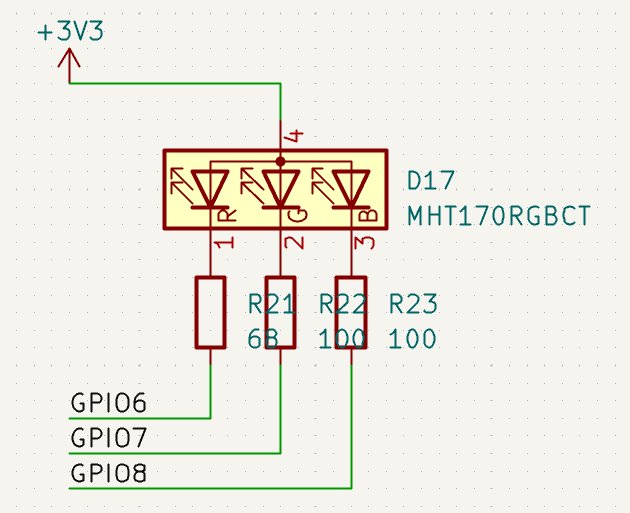
\includegraphics[width=\textwidth-3 cm]{pictures/RGB LED.png}
    \caption{RGB LED [vlastní]}
\end{figure}

Takto je proud a napětí počítány exaktně ze zdroje a piny jsou využívány jako zem. Kvůli konstrukci GPIO pinů, při uzemnění již nejsou problémy se skrytými rezistory. Přemýšlel jsem i jiných řešeních RGB diod, ale toto řešení mi přišlo nejjednodušší. 

\subsection{Komunikace}
Máme dvě komunikační zařízení a potřebujeme vytvořit komunikaci mezi nimi. Komunikace je řešena přes comporty. Hostitel, v tomto případě počítač, na kterém běží hlavní program, si nechá pomocí nástrojů knihovny serial vypsat všechny rozpoznané comporty. Následně se pokusí otevřít comport a poslat mu příkaz. Pokud se mu nepovede otevřít comport, víme že je to nechtěné zařízení. Když se otevření povede, pošle mu příkaz "type". Pokud je na druhé straně správné zařízení neboli klíč se správným nahraným programem, tak zpátky odešle zprávu "player". Jenom tehdy je zařízení dáno do listů zařízení, se kterým potom program pracuje dál.

Hostitelský program je o dost složitější než ten na klíči. Hostitel musí zprávu nejdřív převést do kódování utf-8 neboli bytes. To je posláno na sériovou linku comportu, který je zrovna otevřený. Pico má práci velmi jednoduší, neboť micropython je schopný číst sériovou linku pomocí příkazu input(). Následně pico kontroluje jakou zprávu dostal vůči svému slovníku. Pokud zpráva odpovídá nějakému příkazu, tak pico navrátí odpovídající hodnoty, jinak jenom pošle zpět že zprávu zaregistroval. Hostitel nyní musí projít zpětným procesem převádění zpět z bytes na string. Pokud pico pošle víceřádkovou správu, tak samozřejmě musí komunikační program převést celé pole, které přečte z comportu. 

\subsection{Datová struktura}
Díky způsobu práce s daty na klíči (nepracuje s nimi přímo uživatel, vše je ovládáno pomocí programu) tak zde může existovat velmi neflexibilní struktura souborů. V rootu musí existovat main.py, který se sám spustí, když se pico zapojí. Zároveň musí být v rootu samotný soubor hráče a jakékoli knihovny, které \textit{main.py} potřebuje. Následně všechny skripty, které jsou specifické vůči hráči, musí být v adresáři player\_scripts. Také zde existuje \textit{config.json} na kterém jsou momentálně uloženy informace o datech, které by se měli ukazovat na klíči. Tyto informace musí mít svůj název a maximální hodnoty, kde syntax maximální hodnoty musí být \textbf{max}\textit{VlastníNázev}.

\begin{figure}[H]
	\subsection{Problém}
	Pro vytvoření desky jsem využil program KiCAD. Během tvorby jsem používal pro součástky kombinaci obecných pouzder a specifických (Ty jsem nalezl většinou na stránkách mouser). Bohužel program KiCAD nemá všechny obecné pouzder udělané podle výrobních konvencí. Pro tranzistor jsem použil pouzdro SOT-23 a program přiřadil na piny popořadě kolektor, báze, emitor. Výrobní konvence ale přiřazují, ve stejném pořadí, bázi, emitor, kolektor. Tudíž jsem byl nucen odletovat smd tranzistory a otočil jsem je o přibližně 135 stupňů.


	\centering
	\begin{subfigure}[b]{0.49\textwidth}
	  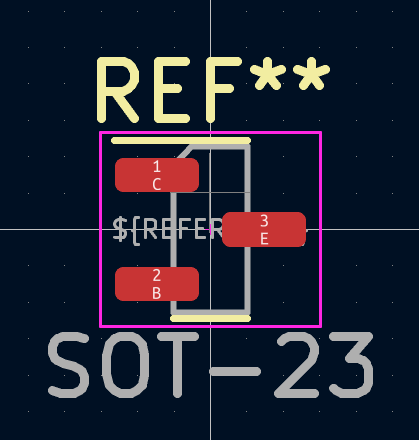
\includegraphics[width=\textwidth]{pictures/wrong_npn.png}
	\end{subfigure}
	\centering
	\hfill
	\begin{subfigure}[b]{0.49\textwidth}
	  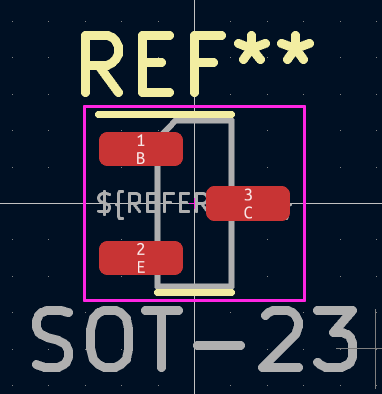
\includegraphics[width=\textwidth]{pictures/right_npn.png}
	\end{subfigure}
	\caption{Špatný a správný tranzistor [vlastní]}
\end{figure}

\section{Hlavní program}
Jakožto vývojové prostředí jsem zvolil Visual Studio Code (Zkráceně VSC), kvůli jeho rozšiřitelnosti. Díky tomu jsem nemusel pracovat ve více různých nástrojů a vývoj proběhl kompletně ve VSC. Druhý důvod byl systém Workspace, který mi umožnil jednoduchý přehled nad všemi adresáři a soubory. Třetí důvod byl jednoduchá integrace s celým systémem git. Tudíž jsem projekty mohl mít uložené na githubu, společně s nastavením VSC, a mohl jsem na práci pracovat kdekoli a kdykoli. Git měl ještě jednu výhodu, a tou je trasování historie souborů. Takto jsem se nemusel bát o žádné mylné smazání nebo přepsání souborů.

Vše je psáno pomocí programovacího jazyka Python, přičemž velmi využívám datového souboru typu json pro ukládání rozmanitých dat. Python je interpretovaný jazyk a tudíž je lehce schopný pracovat se skripty. Zároveň má velmi silné schopnosti zpracování dat. Toto vede k jednoduchosti při psaní a navrhování kódu. Díky jeho minimálnímu syntaxu bylo velmi jednoduché opravovat části dříve psané a prototypovat nové změny. 

Většina her má více části než jednu. V mém případě se program dělí na chytře hloupý hlavní program a nespočet skriptů. Chytrý je protože je schopný, skripty hledat, volat, předávat jim informace co potřebují atd. Hloupý je, protože dělá přesně to co mu uživatel řekne. Tudíž je jeho operace velmi náchylná na chyby způsobené uživatelem.

\begin{figure}[H]
    \centering
    \includegraphics[width=\textwidth-3 cm]{pictures/.png}
    \caption{RGB LED [vlastní]}
\end{figure}

\subsection{Struktura souborů a složek}
Během tvorby programu byl kladen důraz na co nejméně vynucené struktury ze strany vypravěče. Hodně problémů jsem tudíž vyřešil pomocí tvorby souborů se specifickými názvy, pro které se program dívá a vytvoří si strukturu cest, se kterou pracuje a podává do dalších funkcí. Je zde ale určitá kultura, kterou bych doporučil při tvoření souborů.

Hlavní adresář příběhu
\begin{itemize}
	\item Soubor s názvem \textit{\_story.txt}
	\item Adresář s inicializačními skripty
	\item Adresář se skripty eventů
	\item Adresář s hráči (může být prázdný, pokud je použit klíč)
	\item Adresář se skripty hráčů 
	\item player\_scripts
	\item další adresáře, které už tvoří vlastní strukturu příběhu
\end{itemize}

Všechny adresáře, které obsahují skripty, musí obsahovat soubor \textit{\_scripts.txt} a \textit{info.json}. První soubor je hledán aby program věděl kde má skripty uložené a druhý soubor obsahuje informace pro program jak se jednotlivé skripty chovají.

Jednotlivé části příběhu, se kterými chceme aby program pracoval, jsou určeny soubory \textit{storypart.json}. Tento soubor obsahuje jednu informaci pro program, "include" určující obsáhnutí při prvotním načtení, a dále jakékoli další informace, se kterými chce následně vypravěč pracovat ve svých skriptech.

Jedno místo kde program nehledá pro \textit{storypart.json} jsou soubory, které začínají tečkou. Jedno fixní pravidlo s mou verzí programu je, že u každého souboru \textit{storypart.json} musí být .orig adresář. V tomto adresáři musí být původní verze mateřského adresáře. Logické skripty přepisují soubory destruktivně (bez možnosti vrácení změn), proto zde adresáře .orig musí být. I kdyby uživatel vytvořil příběh bez logických skriptů, tak po splnění všech eventů v rámci jedné příběhové části přepíše hodnotu na klíči "include" v \textit{storypart.json} na "false". Toto je moje metoda jak vytvořit pseudo uložení hry. Má to ale stejný problém jako logické skripty, jedná se o destruktivní změny.
\subsection{Handler}
Nejdůležitější součást programu je handler. Tato funkce je schopná vzít script a odpovídající parametry, dosadit hodnoty z paměti, funkci zavolat a uložit její návratovou hodnotu. 

Handler jako funkce má dva svoje parametry. První parametr musí být název skriptu bez koncovky .py (takto jsou uloženy v naimportovaných skriptech). Druhý parametr je pole argumentů, které chceme do funkce poslat. Handler používá vybalovací znaménko * aby první dimenze pole byla předána funkci jako jednotlivé parametry. Zároveň se v této první dimenzi hledá \& znak, který jsem zvolil jako identifikátor že je třeba vzít hodnoty z paměti. Pokud nějakou najde hodnotu v paměti, nahradí \& znak odpovídající hodnotou.

Dalším krokem je zavoláním funkce. Hlavní program obsahuje list importovaných funkcí, a protože Handler žije uvnitř hlavního programu, tak může sáhnout do tohoto listu a funkci zavolat. Volání funkce je provedeno přes funkci getattr().

Zpracování návratových hodnot vyžaduje správné zapsaní informací v \textit{info.json} souborech, které si program načte do paměti. Tyto soubory mají strukturu slovníku a obsahují dvě sekce. První sekcí, jménem id, je soupis názvů skriptů a jejich id. Druhá sekce, jménem info, je určená jak pro důležité programové informace tak pro uživatelské. Dva programové listy které se zde nacházejí jsou pod klíči "func" a "obj". Každá funkce se musí nacházet v jedné z nich a ne v obou zároveň. Handler zjišťuje jestli funkce vrátila hodnotu, pokud ano tak ji ukládá do paměti. Pokud ale skript neobsahuje funkci, obsahuje objekt, tak handler zavolal konstruktor a musí se tudíž celý objekt uložit do paměti.

Mezi další, již nepovinné, informace patří například listy pod klíči "lock" a "logic". První pole říká handlerovi aby hodnotu, kterou načetl z paměti nezahazoval a ponechal ji v paměti. Jsou to tudíž "zamčené" hodnoty. Tato možnost by měla být použita pouze pro skripty u kterých víme že nebudou volány více než jednou. Nebo pokud víme že následně v eventech budou hodnoty násilně požrány. 

Druhý list určuje takzvané logické skripty. Pokud je jejich návratová hodnota typu slovník, mají schopnost přidávat eventy a tudíž jsou logické skripty schopné vytvářet smyčky. Kromě návratových hodnot typu slovník handler také u rozpoznává stringy s koncovkou .json. Pokud je takový string nalezen, tak Handler z odpovídajícího souboru vezme eventy a přidá je. Handler je ještě schopný nalézt jeden identifikátor, "self". Pokud je "self" nalezen a jeho hodnota je true, tak handler přidá, celý původní script, který byl volán. Toto umožňuje snadno vytvořit nekonečnou smyčku.
\subsubsection{Paměť programu}
Struktura paměti je takzvaný stack. Pro tento účel jsem vytvořil třídu, abych si mohl dodat manipulační metody, které bych mohl potřebovat. Samotný stack má strukturu listu (toto jsem zvolil abych mohl použít indexované hledání, mazání, či přidávání hodnot), kdy hodnotou listu je vždy list o dvou hodnotách. Na první pozici stojí vlastní hodnota a na druhé stojí id, neboli adresa, funkce či objektu, co tuhle hodnotu vytvořila. Pokud funkce chce pracovat s hodnotami jiných funkcí, tak je použita první nalezená hodnota "shora" (Pokud bychom se dívali na hodnoty od indexu 0 až do X, tak by to byla první hodnota nalezená od nuly).

Pro manipulaci hodnot jsem vytvořil také dva skripty, které může uživatel používat a to je putVal, pushVal a eatVal. PutVal jednoduše přidá hodnotu do stacku pod svojí vlastní ID. PushVal je schopný posunout hodnotu na na další místo ve stacku za nejbližší hodnotu se stejnou adresou. EatVal požere hodnotu ze stacku i za možnosti že je to "uzamčená" hodnota.

Jak jsem již zmiňoval v sekci Handler, pro čtená z paměti jsem vybral znak \&. Inspiroval jsem se z programovacího jazyka C kde \& operátor vrací adresu proměnné. V mém případě je za znakem \& adresa kde se hodnota má nacházet v paměti.
\subsubsection{Struktura Scriptu}
Kvůli použití funkce getattr() ve funkci Handler, a zjednodušení programu, má script jedno nutné
pravidlo, které se musí dodržovat. Script vždy musí obsahovat stejnojmennou funkci jako soubor, ve kterém je obsáhlá. Na první pohled se toto zdá jako divné pravidlo a vytvoří to velmi elegantní zápis: 
\begin{lstlisting}[language=Python] 
volana_funkce = getattr(importy[funkce],  funkce) 
\end{lstlisting}
\subsection{Okno Hry}
Zobrazování hry jsem se rozhodl použít příkazový řádek. Avšak oproti normálnímu příkazovému řádku, je tento schopný dodržet šířku a výšku okna, udanou v počtu vykreslených znaků. V rámci těchto limitů respektuje slova, tudíž se nikdy nestane, že by bylo slovo odříznuto, nebo vykreslena neúplná věta.

Další funkčnost, kterou toto provedení okna obsahuje je pomalý a rychlý výpis. Celé okno je po každém kliknutí enter překresleno. Informace, které již na obrazovce byly, jsou vykresleny rychle (po slovech) a informace, které jsou nové, jsou vykresleny pomalu(znak po znaku). Konečný efekt, pokud je počítač dostatečně rychlý, vypadá jako kdyby se pouze poslední řádka překreslovala. 

Zde bych rád zmínil, pokud bych další pokračování mé práce zaměřil čistě na grafickou složku, tak bych byl schopný odstranit momentální problém s cenou na výkonu. V této práci jsem toho nebyl schopný, protože s mými znalostmi, v rámci této práce, bych při vytvoření takového okna byl nucen použít velký počet proměnných, které by mi dávali informace o momentálním stavu okna. Řádná optimalizace by vyžadovala mnohem složitější funkci a nebo bych přešel na systém vytvoření okna, které by simulovalo chování příkazového řádku. V případě nového okna by optimalizace byla zajištěna grafickým enginem, který bych používal pouze k vykreslování textu.
\subsubsection{Logické provedení}
První co se musí provést, z kterékoli části programu, je metoda add\_text. Ta je schopná přijmout dva možné vstupy. Buď přes list, pole, nebo jiné iterovatelné objekty, nebo přes string. Pokud je přijat iterovatelný objekt, tak je každá hodnota braná jako string a přidaná do paměti okna, pokud je přijat string tak je přidán do paměti rovnou. Než ale se cokoliv přidá, tak projde kontrolou, jestli je možno takovou větu vykreslit. Pokud řádka projde skrz kontroly, tak je přičtena jednička k proměnné, která řídí postupné vykreslování.

\begin{figure}[H]
    \centering
    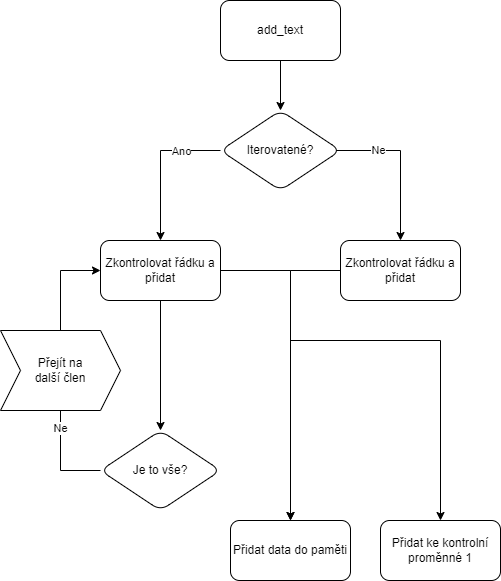
\includegraphics[width=\textwidth-3 cm]{pictures/logic-window.drawio.png}
    \caption{Diagram přidání dat do okna[vlastní]}
\end{figure}

Ve skriptech jsem vytvořil ještě jeden, rozšířující, skript. Je stejnojmenný jako metoda okna pro přidání textu, ale je schopný vzít txt soubory. Skripty mají přístup k adrese, pokud si ji vyžádají, kde momentálně mají pracovat. Při použití tohoto skriptu je důležité brát na vědomí, že skript pro textové soubory hledá v adresáři \textit{texts}, v pracovní cestě.

Vykreslování samotné je tvořené přes dvě metody. Jedna metoda jenom připravuje pole, které vykreslovací metoda dá do okna. Vykreslovací metoda neobsahuje žádnou logiku jestli může nebo nemůže vykreslit něco na obrazovku, vše zařizuje formátovací metoda.
Formátovací metoda pomalu postupuje skrz paměťový list a prochází skrz něj odshora dolů.
\subsubsection{Formátování}
Jak jsem již zmínil tak formátování je schopné dodržovat velikost okna. Kromě toho ale umí pracovat i se speciálními znaky. Momentálně implementované znaky jsou <h>, <un> a <r>. Syntax těchto znaků je převzatý z tagů v HTML. <h> a <un> jsou znaky, které jsou "hookovací", což zde znamená že jsou schopné připnout řádku k vrchu formátovaného okna. Připnuté řádky budou připnuté tak dlouho dokud se přímo pod nimi neobjeví řádka s <un> znakem. Takto se dá připnout kolik řádek je potřeba, ale program nepustí text do paměti, pokud by připnuté řádky zaplnili okno úplně. Poslední znak <r> je určený pro započetí čtení z příkazového řádku.

Řádky v paměti nejsou rozřezány podle šířky okna takže se musí se zalomením textu počítat při formátování. Jako správné chování programu jsem uznal, že pokud je textu enter, tak ho to vykreslí. Samozřejmě při přidávání textu do paměti se kontroluje aby vůbec řádka bylo možno ji celou dostat na obrazovku. Formátovaní slov na kraji obrazovky jsem vyřešil tak že jsou posunuty na další řádek.
\subsubsection{Vytváření a práce s oknem}
Okno se vytvoří přes event, kdy parametry eventu jsou šířka a výška okna. Jak jsem již zmiňoval v Handlerovi tak okno je uloženo do paměti, jako objekt, protože Handler zavolá konstruktor. U okna silně doporučuji hodnotu dát mezi "uzamčené" hodnoty, aby po každém podání okna eventu, nebylo zničeno.

Jak už jsem zmínil v sekci logické provedení, tak pro přidání textu do okna se dá použít buď přímo metoda objektu, nebo stejnojmenný skript. Pokud je skriptu povolen přístup k objektu, tak je teoreticky schopný ovládat rendrování do okna přímo. Jedna z hlavních věcí co ale okno umí je zapnout automatický render. Opět se dá spustit přes metodu nebo přes skript. Objekt má metodu jak pro zapnutí tak pro vypnutí, ale skript přepíná mezi zapnutým auto renderem a vypnutým. 

Auto render má ještě jednu hlavní vlastnost a to že spustí vykreslování okna na jiném vlákně než hlavní smyčka. Umožňuje to přidávat text a procházet neblokující eventy i když uživatel nic nedělá, ale vytvořilo to lehké potíže při tvoření čtení dat.

\subsubsection{Input}
Jak již bylo zmíněno, tak okno je schopno rozpoznat tag <r> a započne čtení. Teoreticky by toto čtená neměl vůbec být problém, ale kvůli použití vláknění to nebylo triviální. Na první pohle by se zdálo že jsem měl použít knihovnu \textit{Asyncio} ale našel jsem, podle mě, lepší řešení. Knihovna \textit{Threading} je schopná tvořit asynchronní input a output, a to díky tomu že sdílí primitivní typ \textit{Future} (V Threading se jmenuje Event). Tento typ funguje tak že po jeho nastavení jsem schopný z různých míst programů "sepnout" tento typ nebo ho "vypnout". Následně je ve funkci možno nastavit aby funkce asynchronně čekala na "sepnutí".

Tuto teorii jsem zkonstruoval na got\_input, což je \textit{Future}, a metoda \textit{get\_return\_value()}, která získává hodnotu z příkazového řádku. Pokud kterýkoliv skript zavolá metodu pro získání hodnoty, tak v ten moment začne čekat dokud uživatel něco nezadá. Okno ale bude čekat než se dostane na řádek s tagem <r>.

Kvůli mému provedení nedoporučuji dávat čtecí tag přímo do textu. Vytvořil jsem skript \textit{ask}, který je schopný nejen získat input, ale je zároveň schopný poslat otázku do okna, přidat k ní možnosti, pokud je uživatel zadá, a dodat nutný čtecí tag. Možnosti, které může uživatel poskytnout eventu \textit{ask}, jsou typu slovník (dict). Klíče jsou nahrány do okna. Hodnoty, potom co si uživatel vybere možnost, jsou vráceny do paměti programu. Tudíž může uživatel pracovat s daty, které se nebudou uživateli zobrazovat. Pokud uživatel zadal hodnotu, na kterou se nikdo neptal, tak \textit{ask} vypíše do okna, že uživatel zadal neplatnou možnost, a zopakuje otázku.
\subsection{Hráč}
Další důležitou částí programu je uložení hráče a představení hráče v programu. Hráč je uložen v \textit{json} souboru a v programu je představen pomocí objektu. Samotný hráč má spoustu parametrů a pár důležitých zmíním. Každý hráč má svoje vlastní identifikační číslo, což je 32 znaků dlouhý hexadecimální text. Pomocí tohoto náhodného identifikačního klíče jsou možné dvě stejně pojmenované postavy, které se ale chovají naprosto jinak. Další místo kde je tento klíč užitečný, je ve skriptech, specifických pro nějakou postavu.

Všechny postavy mají skripty, které jsou jim přístupné. Jsou to skripty jako přidání věcí do inventáře nebo odebrání věcí z inventáře. Takové skripty jsou nutné aby existovali pro všechny. Pokud ale bude jedna z postav třeba Berserk a má mít schopnost tak silného úderu, že zároveň zraní sám sebe, tak je to možné vytvořit přes ID. 

V rámci věcí co jsou nutné mít v každém hráči, je to pouze ID a type. Všechno ostatní je už specifické vůči mému provedení hráče.

\subsection{Eventy}
Během předchozích textů jsem zaměňoval slova event a skript. Event je přepis pro hlavní program aby byl schopný pustit skript. Skript je podprogram, který hlavní program používá pro své akce. Přepis jednotlivých eventů je v souboru \textit{event.json}, který se musí nacházet na úrovni \textit{storypart.json}.

Samotný zápis je syntax json slovníku. Klíčem je název skriptu, který chce uživatel použít, plus \_X, kde X je pořadí eventu v momentálním souboru. Část \_X je zde jenom kvůli tomu, že klíče nemohou být stejné. Hodnotou ke klíči je vždy pole argumentů, které Handler podá skriptu. Zde se píší již zmiňované znaky \& aby byla umožněna komunikace mezi skripty.

\begin{figure}[H]
    \centering
    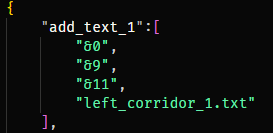
\includegraphics[width=\textwidth-3 cm]{pictures/event.png}
    \caption{Ukázka zápisu eventu [vlastní]}
\end{figure}
\section{Skriptovací nástroj}
Když si shrneme co by vše uživatel musel umět aby si příběh napsal, tak by to znamenalo, že je nejspíš programátor a může si tudíž klidně naprogramovat vlastní hru. Tudíž jsem se rozhodl udělat nástroj, který by byl schopný pomoct uživateli a dát mu inteligentní předpovídání při psaní eventů a jiných souborů. Stejně jako hlavní program, tak skriptovací nástroj obsahuje vlastní verzi Handlera, díky které se opět stává kompletně rozšiřitelný. Bohužel ale není naprosto kompletní, nepatří mezi hlavní části mé práce, ale i tak mi přišlo ho do určité míry připravit.

Nástroj je opět v příkazovém řádku ale oproti Hlavnímu programu je jeho výpisová schopnost vyšší. Má sice jeden zásadní problém ale k němu se vyjádřím později.

\subsection{Forma}
Tento nástroj jsem chtěl zpracovat jako můj vlastní příkazový řádek, s možností do něj přidávat nástroje. Samozřejmě byl zamýšlený k práci se hrou, ale teoreticky nic nebrání tomu, aby kdokoli použil tento řádek na cokoliv jiného. 

Když jsem začal nástroj dělat, tak jsem uměl víc pracovat s řádkem než když jsem začal dělat původní hru. Tudíž jsem byl při tvoření vytváření vykreslování odvážnější a umožnil jsem jiné další věci, které hra vůbec neumí. Jednou z nich je nabídka možností uživateli co doplnit za název skriptu. Aktivuje se zmáčknutím klávesy šipka nahoru. Handler zařídí aby program věděl jaké věci navrhnout. Následně může uživatel šipkami vlevo a vpravo navolit, kterou možnost chce použít. Klávesou TAB se možnost vepíše do řádku. Pokud by uživatel chtěl volbu zrušit, tak může pomocí šipky dolů. Nabídka slov se ještě navíc ukazuje v modrém. Všechny tyto implementace jsou díky dvěma znalostem. První je znalost knihovny keyboard, která mi nesmírně pomohla, a druhá je znalost ASCII escape sekvencí.

Řádka má dva příkazy vestavěné do programu. První je \textit{cd} a druhý je \textit{cls}. Tyto příkazy kopírují funkce klasického příkazového řádku windows, tudíž \textit{cd} umožňuje uživateli přepínat mezi adresáři a \textit{cls} vrátí příkazový řádek do původního stavu. Další příkazy, které jsou všestranné, jsou příkazy ze skriptu \textit{list\_all}. Tento soubor obsahuje příkazy \textit{ls, ld, lf, list\_all, list\_dir, list\_files}. \textit{List\_all} a jeho krátká verze by měla napovědět její funkci. Vypíše vše co obsahuje adresář. Další dvě možnosti příkazů vypíšou pouze adresáře nebo pouze soubory. Adresáře jsou zabarveny modře a soubory červeně. U souborů je ještě za svislou čárou napsaná jejich velikost.
\subsection{Handler}
Podobně jako Handler v hlavním programu, je tento Handler schopný volat skripty a podávat jim argumenty. Má ale mnohé změny. Prví nastanme rovnou přímo při importování programu. Skriptovací nástroj má fixní strukturu souborů. Což v tomto případě znamená, že všechny skripty musí existovat na úrovni \textit{main.py}. 

První změna je celkem regresivní, další byly podle mě vylepšení oproti Handlerovi hlavního programu. V každém skriptu musí existovat funkce get\_attr(), která vrací informace pro Handler. Návratová hodnota je slovník, který v klíčích obsahuje názvy funkcí, které skript obsahuje. V hodnotě se nachází list, který obsahuje list a string. V listu jsou možnosti, které může nástroj předložit uživateli jako možnosti, a které následně podá funkci zpět. String je zde pro případy jako  \textit{\_\_local\_files\_\_}, pokud by nebylo možno napsat možnosti. Víceméně chybová zpráva. Pokud by script potřeboval uživateli předložit soubory v aktuálním adresáři, tak stačí do návratové hodnoty vložit již zmíněné \textit{\_\_local\_files\_\_}.

\subsection{Nástroj edit a create}
Zprvu jenom chci říct, že nástroj \textit{create} nedělá nic převratného. \textit{Create} vytvoří soubor a následně zavolá edit nástroj.

Nástroj edit je jeden z mých největších skriptů a bohužel je velmi nekompletní. Momentálně je schopen editovat klasické textové soubory, a umí chytře pomáhat při tvorbě eventů. 

První co se tvůrci skriptu zobrazí je vzhled souboru v momentální verzi. Šipkami nahoru a dolu se mění výběr řádku, se kterým potom může tvůrce pracovat. Pokud zmáčkne klávesu \textbf{n} tak se pod momentálně zvolenou řádkou přidá nová prázdná. V moment co se uživatel dostane do tvoření řádku, tak může uživatel vyvolat pomoc šipkou nahoru. Objeví se modře zabarvený text. Šipkami doleva a doprava se mění momentální možnost. Zmáčknutím klávesy \textbf{TAB} se zvolí možnost a vypíše se do řádku. Klávesa delete nebo šipka dolů zavře nabídku.

Ze základu jsou v nabídce některé časté znaky co jsou často potřeba při tvorbě souborů json. Příkladem jsou hranaté a složené závorky. Pokud se uživatel ocitne mezi uvozovkami, tak se nabídka rozšíří o všechny skripty v hlavním programu. Skripty jsou adekvátně očíslovány a uživatel může vybrat který skript chce použít.

Když je uživatel s řádkem hotový tak klávesou enter řádku vloží do nabídky. Klávesa \textbf{r} potvrdí jestli je momentální verze souboru validní json soubor, pokud ne tak označí řádku, kde byla nalezena chyba. Klávesou \textbf{s} se soubor uloží, a tvůrce je navrácen do hlavního příkazového řádku.

Největší problém, který zůstává nevyřešený je, že tvůrce pořád potřebuje velké množství znalostí o skriptech, které se nedají zjistit bez znalosti jazyka Python. Další problém je že aby byla implementace kompletní, tak je potřeba přidat možnost tvorby souborů hráče a souborů s informacemi o skriptech.
\subsection{Nástroj auto\_script}
Tento nástroj, podobně jako nástroj edit, je ve velmi raných verzích. Tento skript by měl pomoct při přiřazování adres do skriptů  a přiřazování skriptů k dodatečným vlastnostem. Momentálně je všeho schopen ale jde o velmi barbarskou ukázku.

Jedna z chytrých věcí co jsem sem přidal je, že skript najde největší momentální adresu v ostatních souborech a zjistí jeho řád. Číslování adres bude buď pokračovat podle poslední adresy v souboru, nebo bude začínat na o jeden vyšším řádu. Pokud by tento nástroj byl použit pči tvorbě celého příběhu, tak by měl zamezit překrývání adres.


\section{Závěr}
Během práce jsem narazil na mnohé problémy a komplikace. Během řešení jsem se naučil mnohé věci a nyní si uvědomuji mnohé nedostatky mé práce. V rámci zadání jsem práci podle mě splnil, ale sám vím že jsou místa, kde by si program zasloužil vylepšení. Mé řešení problému má podle mě dobrý základ a chci s ním dál pokračovat. Jednu věc co jsem v tomto rámci také poznal je, že buď budu pokračovat ve tvorbě klíče, nebo ve tvorbě hry. Tvorba obou zároveň ranila kvalitu obou. Také jsem pro příště poučen a pokud se pustím do tvorby her, tak musím práci více rozkouskovat. Kvůli mé relativní nezkušenosti na začátku jsem si ani neuvědomoval kolik práce zabere postavit hru od začátku až do konce, a natož ještě hru, která je skriptovatelná.

Největším momentálním problémem je bohužel použití jazyka Python. Tento jazyk je velmi flexibilní a pomohl při zpracování dat a vypisování dat na obrazovku. Problém ale je jeho optimalizace. Na problémy s rychlostí jsem narazil z jedné části, protože nepíši absolutně optimalizovaný kód, a z druhé. Ta druhá je, že je jazyk Python interpretovaný, ne compilovaný. Toto má i druhý nešťastný efekt, a to je že program lze spustit u uživatele jenom tehdy, má li nainstalovaný Python a jeho knihovny.

Do budoucna počítám že celý program přenesu na jazyk, který má přímo compiler nebo JIT a který je schopné této kompilace na jakýkoliv operační systém. Musím se přesunout k mnohem méně dynamickému typování, protože to vytvořilo mnoho chyb. Musím také do programu vnést víc asynchronního chování a lepší souborovou strukturu. Chci zanechat dynamické hledání věcí ale co nejvíc věcí, které se dají vypočítat předem, tak by měli být uloženy do souborů s nějakou fixní adresou. Dynamické hledání je příjemné pro tvůrce, ale zpomaluje program. Tudíž by měli existovat adresáře a soubory, se kterými tvůrce nemá pracovat a ve kterých jsou uloženy výsledky výpočtů.

Vykreslovací okno bylo vytvořeno během raných začátků programu. Tudíž je velmi náročné na procesor, nemá dobré schopnosti s grafikou a jeho jediná opravdová schopnost je vykreslovat rychle a pomalu. Vykreslování ve skriptovacím nástroji je lepší, ale stálo to ještě víc výkonu než původní okno. Obojí je potřeba předělat, a to nejlépe do grafického enginu, který bude optimalizovaný pro práci s textem a vstupní příkazovou řádkou. Musí také obsahovat lepší rozpoznání šířky okna a práci s řádky. Momentálně se všechny moje funkce rozpadnou v moment co je okno menší, než skripty očekávají. Líbí se mi že je program v rámci příkazového řádku, a budu se toto i nadále snažit ponechat, potřebuji ale více logiky a optimalizace. Také by engine měl obsahovat schopný text parser, aby vstupy uživatele mohly být volnější a negenerovali tolik chyb.

Struktura skriptů musí též dostat předělání. V rámci programu musí být lepší nahrávání informací ohledně skriptů a musí být podporována volnější struktura vnitřního vzhledu skriptu. Ve skriptovacím nástroji jsem byl schopný některé tyto problémy vyřešit, ale pořád to není dostatečné.

Dynamičnost programu na klíči se také musí zlepšit. Momentálně je program a hlavně slovník naprogramovaný tvrdě. Toto není podle mě dobré řešení a bylo by lepší abych vytvořil podobný systém jako na počítači pro jednoduché rozšiřování slovníku.

Během pracování s deskou jsem narazil na problém. Kvůli časovému multiplexu jsou LED schopné svítit pouze na 50~\% což není ideální při přihlédnutí k velikosti a svítivosti LED. Během přemýšlení o tomto problému mě napadlo lepší řešení při použití stejného počtu pinů a to za použití dvou paralelních registrů. Díky těmto dvěma registrům můžu posílat nové informace na LED pouze když se změní. Toto by LEDkám umožnilo svítit na 100~\%. Toto řešení má jednu nevýhodu a to je že má vyšší počet součástek.

%\subsection{Problémy}
%\subsection{Budoucí řešení}
%\subsubsection{Hlavní program}
%\subsubsection{Skriptovací nástroj}
\section{Zdroje}
Draw.io - free flowchart maker and diagrams online. Flowchart Maker \&amp; Online Diagram Software [online]. [Accessed\&nbsp;12\&nbsp;April\&nbsp;2023]. Available from: https://app.diagrams.net/ 
\section{Přílohy}
\end{document}